\documentclass[xcolor=dvipsnames]{beamer}
\usetheme{CambridgeUS}
\usepackage{graphicx}
\usepackage[tableposition=top,font=tiny,labelfont=tiny]{caption}
\beamertemplatenavigationsymbolsempty
\usepackage[loadonly]{enumitem}
\newlist{arrowlist}{itemize}{1}
\setlist[arrowlist]{label=$\Rightarrow$}




\newcommand{\testIt}[1][A text that can be changed locally\ldots]{Project: Heartdisease}
\author{Öcal K., Pavlo N., Sunyoung JI}
\title{Statistical Learning}
\date{16.09.2022}

\begin{document}


\begin{frame}[plain]
\vspace{-0cm}
\begin{center}
  \makebox[\textwidth]{
\includegraphics[scale=0.4]{duelogo_en.png}}
\end{center}
\vfill\vfill
\begin{center}
{\Large Statistical Learning}
\vfill
{\large \testIt}
\vfill\vfill
{\large Öcal Kaptan(TU), Pavlo Nikitenko(UDE), Sunyoung JI(TU)}\\

{\small University of Duisburg-Essen}\\

{\small 16.09.2022}
\end{center}
\end{frame}\addtocounter{framenumber}

\begin{frame}
\frametitle{Overview}
\begin{enumerate}
\item Introduction
\item Pre-Processin
\item Model Selection and Training
\item Modelling Approach 
\begin{itemize}
\item a) Logistic Regression
\item b) Discriminant Analysis
\begin{itemize}
\item LDA
\item QDA
\item FDA
\end{itemize}
\item c) Tree-Based Methods
\begin{itemize}
\item Decision Trees
\item Gradient Boosting Machine
\item Random Forest
\end{itemize}
\end{itemize}
\item Conclusion
\end{enumerate}
\end{frame}

\begin{frame}{1.Introduction}
\begin{itemize}
\item Aim is to analyze the "Heart" dataset and make predictions of the HeartDisease status of a person. So we try to find a statistical learning models which classify if a person has heartdieseas ("Yes") or is healthy ("No")
\item We consider the folliwing Supervised Methods for classification problems: Logistic Regression, Discriminant Analysis and Tree-Based Methods.
\item We split the dataset into a training and test dataset (80/20)
\item To asses the models we consider the accuracy (correctness rate), True Positiv Rate (TPR=How many of true "Yes" are predicted right), True Negative Rate (TNR= How many of true "No" are predicted right) and the rate of Area under the Curve (AUC for comperison how good the model performs).
\item To tidy up the dataset we pre-processed the data in Section 2.
\item We test different approaches to reduce the model complexity to overcome overfitting and optimize the bias-variance trade-off. 
\end{itemize}
\end{frame}


\begin{frame}{2.Data Pre-Processing}
The data inlcudes 19 (with the response HeartDisease) predictors with 287816 individuals (observations). There are 12 Nominal Variables with different Levels, 5 Numeric and 2 Ordinal Variables. So we made the follwing Steps to tidy up the dataset:
\begin{itemize}
\item Removed one predictor (X) which was a random vector with numbers without any meaning for the heartdisease status.
\item Checked the missing values.
\item Each variables was checked in respective probability of having Heartdisease, removed "AlcoholDrinking" and "Race".
\item Better understanding of each variables and classes, we used some transformations:
\begin{itemize}
$\Rightarrow$ \textbf{AgeCategory} (which has 13 levels) is converted to 3 classes which are “Youth”,“Adults” and “Seniors”.

\newline $\Rightarrow$ \textbf{GenHealth} is coverted to 4 classes which are "Poor","Fair","Good", "Excellent".

\end{itemize}
\end{itemize}
\end{frame}


\begin{frame}{2.Data Pre-Processing}
\begin{itemize}
\begin{itemize}
$\Rightarrow$ \textbf{MentalHealth} converted to 3 classes which are "Bad","Fair","Good".

\newline $\Rightarrow$ \textbf{BMI} and \textbf{SleepTime} normalized.
\end{itemize}
\item Convert all the character types of variables into factor. 
\item Convert all factor predictors to dummies (In total 23 Predictors, each level is one predictor)
\item Checked colliniarity
\end{itemize}
\end{frame}

\begin{frame}{3.Model Selection and Training}
\begin{itemize}
\item In this section dataset splitted into traning and pre-test part (80/20). After the seperation, \textbf{regsubsets()} function used on training data set to find best parameters for the models.

\begin{figure}
    \centering
    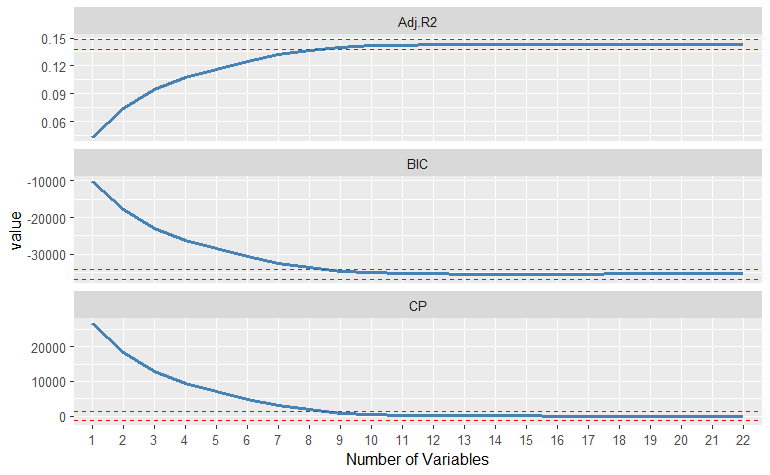
\includegraphics[scale= 0.45]{regsubset.png}
    \caption{Example forward best parameter via R2, BIC and CP Criteria}
    \label{fig:my_label}
\end{figure}
\end{itemize}
\end{frame}

\begin{frame}{3.Model Selection and Training}
\begin{itemize}
\item We used forward, backward and Normal subset selection and get eleven predictors:
\begin{figure}
    \centering
    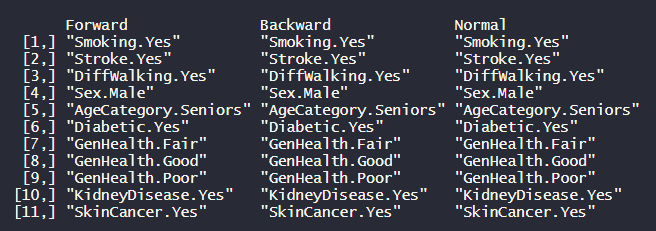
\includegraphics[scale= 0.5]{bestSubset.png}
    \caption{best parameter via subset selection}
    \label{fig:my_label}
\end{figure}
\item All methods selected the same best predictors.
\end{itemize}
\end{frame}

\begin{frame}{4.Modelling Approach}
\begin{itemize}
\item For the  modelling approach, upsampling method is used with  repeated cross validation. 
\item Upsampling methods replicates the observations from minority class to balance the data.
\item  Also, \textbf{Repeated Cross-Validation} is used with  3 times repeat and 10-fold to find the optimal modell.
\end{itemize}
\end{frame}

\begin{frame}{4a.Logistic Regression}
\begin{itemize}
\item Logistic Regression ensures that our estimate lies between 0 and 1.
\item Moreover, logistic regression uses Maximum likelihood to seek estimates which corresponds as closely as possible to the
individual observed HeartDiesease levels.
\item  The likelihood gives the probability of the observed
zeros and ones in our case and finds estimates to maximize the likelihood of the observed data.
\item For logsitc regression we used the 11 best predictors chosen by susbet selection. 
\item As performance measure is used not only the accuracy rate, but also True Postiv Rate (TPR), True Negative Rate (TNR) and Area under the Curve (AUC).
\end{itemize}
\end{frame}

\begin{frame}{4a.Logistic Regression}
\begin{itemize}
\item After building the model and fit on \textbf{train data set}, the accuracy of the final model is about 75,5\%.
\item  The TPR (how many Yes's we predicted rigth) is 74,7\%. 
\item The TNR (how many NO's we predicted right) is about 75,6\%.
\item The AUC (Are under the Curve) is 82,5\%.
\newline \textbf{It seems to be that the best logistic regressions performs very well for both levels and we have a really high AUC.}
\end{itemize}
\end{frame}

\begin{frame}{4a.Logistic Regression}
\begin{itemize}
\item Now use the \textbf{new test data set} wtih our model. Before we do all the transforamtion steps mentioned in \textbf{Section two}
\item The new dataset has 31979 observatons and 23 predictors.
\item We get with the new test dataset:
\begin{itemize}
$\Rightarrow$ Accuracy 75,5\%
\newline $\Rightarrow$ TPR 73,9\%
\newline $\Rightarrow$ TNR 75,6\%
\newline $\Rightarrow$ AUC 82,2\%
\end{itemize}
\textbf{So we get a really good performance on the new unknow data set to correctly predict both levels of the heart disease.}
\end{itemize}
\end{frame}

\begin{frame}{4b.Discriminant Analysis}
For discriminant analysis 3 models are used as below:
\newline \textbf{Linear Discriminant analysis (LDA)}
\begin{itemize}
\item LDA assumes that predictors are normally distributed  (Gaussian distribution) and the different classes have class-specific means and equal variance/covariance.
\item The accuracy for LDA by using the predictors from subset selection  process obtained as 74\%.
\item But when we tried to use LDA on full dataset and remove the unsignificant predictors, we achivied 76\% of accuracy.
\item That's why subset selection is not used for LDA.
\end{itemize}
\end{frame}

\begin{frame}{4b.Discriminant Analysis}
\textbf{Quadratic Discriminat Analysis (QDA)}
\begin{itemize}
\item QDA is little bit more flexible than LDA, in the sense that it does not assumes the equality of variance/covariance.
\item In other words, for QDA the covariance matrix can be different for each class.
\item For QDA the predictors from subset selection process are used. QDA get a accuracy of 81,72\%
\end{itemize}
\textbf{Flexible Discriminant Analysis (FDA)}
\begin{itemize}
\item FDA is a flexible extension of LDA that uses non-linear combinations of predictors such as splines.
\item FDA model get a accuracy of 76,40\%.
\end{itemize}
\end{frame}

\begin{frame}
Collect all results for \textbf{train data set} the three models in a plot we get:
\begin{figure}
    \centering
    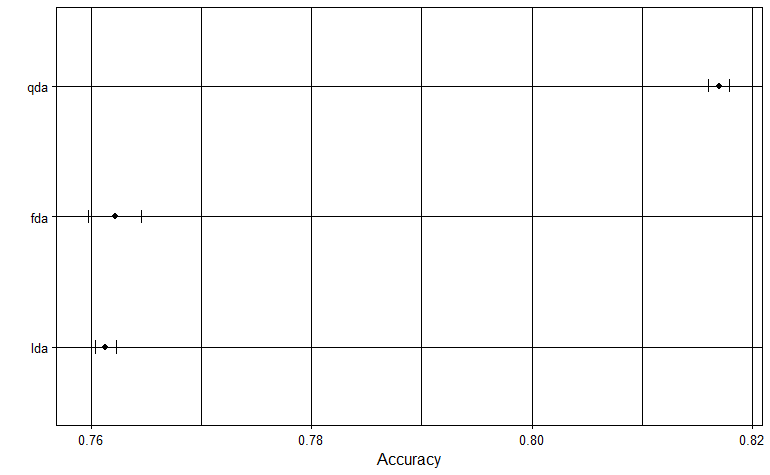
\includegraphics[scale= 0.45]{QDA_FDA_LDA.png}
    \caption{Accuracies for LDA, QDA and FDA}
    \label{fig:my_label}
\end{figure}
\end{frame}

\begin{frame}{4c.Tree-Based Methods}
\textbf{Decission/Classification Tree}
\begin{itemize}
\item This method involves segmenting the predictor space into a number of single regions.
\item Since the set of splitting rules used to segment the predictor space can be summarized in a tree.
\item It is important to find the optimal tree size, since a to large tree with to many splits overfits the data and performances bad on the test dataset.
\item Fit on a \textbf{train data}, the optimal CP choosing by 3x10 CV is 0.001 and give the follow tree:
\end{itemize}
\end{frame}

\begin{frame}{4c.Tree-Based Methods}
\begin{figure}
    \centering
    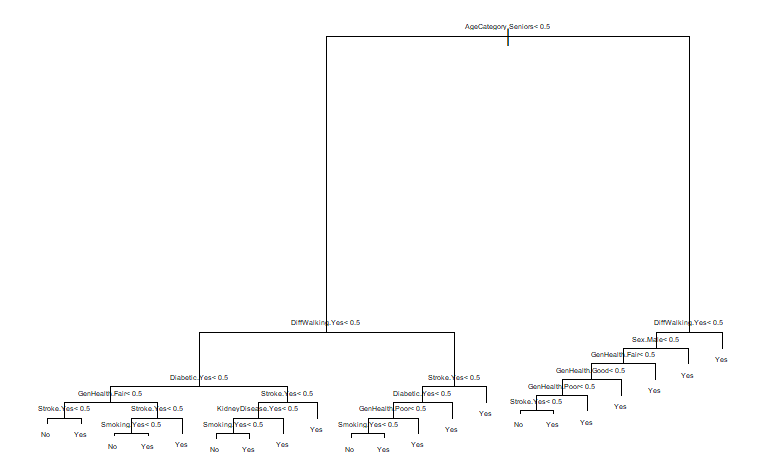
\includegraphics[scale= 0.6]{Decision_Tree.png}
    \caption{Best purned Tree}
    \label{fig:my_label}
\end{figure}
\end{frame}

\begin{frame}{4c.Tree-Based Methods}
\begin{itemize}
\item The devision of nodes indicates that Age, DiffWalking, Diabetic, Sex, Stroke, Smoking, KidneyDisease and general health seem to have high importance for assessment of a persons Heart disease status.
\item the Accuracy of the best tree model is about 70,3\%.
\item The TPR (how many Yes's we predicted right) is 80,5\%.
\item  The TNR (how many No's we predicted right) is about 69,4\%. \item The Are under the Curve is 79,2\%.
\end{itemize}
\end{frame}

\begin{frame}{4c.Tree-Based Methods}
Now use the \textbf{new test data set} with our best tree model and get:
\begin{itemize}
\item Accuracy 70,1\%
\item TPR 79,5\%
\item TNR 69,2\%
\item AUC 78,7\%
\end{itemize}
So we get a really good performance on the new unknow data set of TPR and a little bit less TNR. 
\newline \textbf{It seems to be that the best classification tree performs slightly worse on train and new test data set than for example the best logstic regression model.}
\end{frame}

\begin{frame}{4c.Tree-Based Methods}
\textbf{Gradient Boosting Machine}
\end{frame}

\begin{frame}{4c.Tree-Based Methods}
\textbf{ Random Forest}
\end{frame}

\begin{frame}{5.Evaluation}
\begin{itemize}
\item Concluding, the models measured on the \textbf{train} and \textbf{new test set}.
\item Performance of the new test set shown below.
\begin{figure}
    \centering
    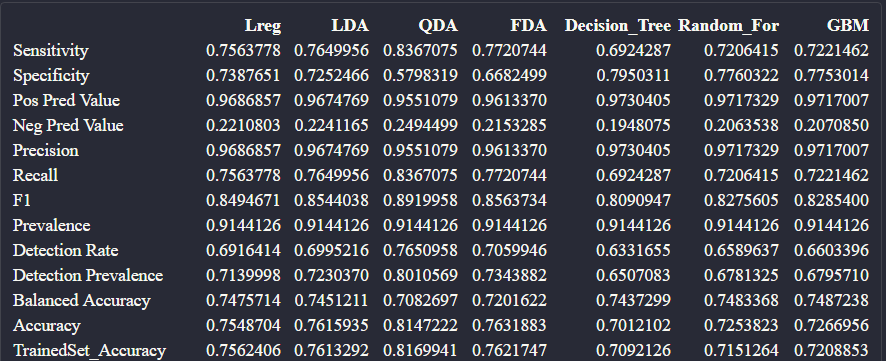
\includegraphics[scale= 0.45]{Evaluation.png}
    \caption{Measures of all models}
    \label{fig:my_label}
\end{figure}
\end{itemize}
\end{frame}


\end{document}